%%%%%%%%%%%%%%%%%%%%%%%%%%%%%%%%%%%%%%%%%

%%%%%%%%%%%%%%%%%%%%%%%%%%%%%%%%%%%%%%%%%

%----------------------------------------------------------------------------------------
%	PACKAGES AND OTHER DOCUMENT CONFIGURATIONS
%----------------------------------------------------------------------------------------

\documentclass[final]{beamer}
\usepackage{bigints}

\usepackage{graphicx} % Required for including images
\graphicspath{{figures/}} % Location of the graphics files
\usepackage{booktabs} % Top and bottom rules for table
\usepackage[font=small,labelfont=bf]{caption} % Required for specifying captions to tables and figures
\usepackage{amsfonts, amsmath, amsthm, amssymb} % For math fonts,  symbols and environments
\usepackage{wrapfig} % Allows wrapping text around tables and figures
\theoremstyle{plain}
\newtheorem{thm}{Theorem}[section]

\newtheorem{prop}[thm]{Proposition}
\newtheorem*{cor}{Corollary}

\theoremstyle{definition}

\newtheorem{conj}{Conjecture}[section]
\newtheorem{exmp}{Example}[section]

\newtheorem{defn}{Definition}[subsection]
\theoremstyle{remark}
\newtheorem*{rem}{Remark}
\usepackage{mathpazo}
\usepackage{mdframed} %Allows text boxes and text background
\usepackage{xcolor}%extends the range of specified colours
\usepackage{float}
\usepackage[scale=1.24]{beamerposter} % Use the beamerposter package for laying out the poster

\usetheme{confposter} % Use the confposter theme supplied with this template
\usepackage{exscale} %allows integrals to be rescaled

\setbeamercolor{block title}{fg=ngreen,bg=white} % Colors of the block titles
\setbeamercolor{block body}{fg=black,bg=white} % Colors of the body of blocks
\setbeamercolor{block alerted title}{fg=white,bg=dblue!70} % Colors of the highlighted block titles
\setbeamercolor{block alerted body}{fg=black,bg=dblue!10} % Colors of the body of highlighted blocks
% Many more colors are available for use in beamerthemeconfposter.sty

%-----------------------------------------------------------
% Define the column widths and overall poster size
% To set effective sepwid, onecolwid and twocolwid values, first choose how many columns you want and how much separation you want between columns
% In this template, the separation width chosen is 0.024 of the paper width and a 4-column layout
% onecolwid should therefore be (1-(# of columns+1)*sepwid)/# of columns e.g. (1-(4+1)*0.024)/4 = 0.22
% Set twocolwid to be (2*onecolwid)+sepwid = 0.464
% Set threecolwid to be (3*onecolwid)+2*sepwid = 0.708

\newlength{\sepwid}
\newlength{\onecolwid}
\newlength{\twocolwid}
\newlength{\threecolwid}
\setlength{\paperwidth}{36in} % A0 width: 46.8in
\setlength{\paperheight}{48in} % A0 height: 33.1in
\setlength{\sepwid}{0.015\paperwidth} % Separation width (white space) between columns
\setlength{\onecolwid}{0.27\paperwidth} % Width of one column
\setlength{\twocolwid}{0.4\paperwidth} % Width of two columns
\setlength{\threecolwid}{0.23\paperwidth} % Width of three columns
\setlength{\topmargin}{-0.5in} % Reduce the top margin size
%-----------------------------------------------------------
\usepackage{environ}
\usepackage{varwidth}
\usepackage{lipsum}
\usepackage{graphicx}  % Required for including images
\usepackage{amssymb}
\usepackage{amsbsy}
\usepackage{mathrsfs}
\usepackage{booktabs} % Top and bottom rules for tables
\usepackage{multicol}
\usepackage[export]{adjustbox}
\usepackage{eso-pic}
\usepackage{mdframed}

%----------------------------------------------------------------------------------------
%	TITLE SECTION 
%----------------------------------------------------------------------------------------
\columnsep=20pt % This is the amount of white space between the columns in the poster
\columnseprule=5pt

%%%%%%%%%%%%%%%%%%%%%%%EDITEDIT
% Fill in the following fields for the title section. 
% To format the display of the title section you will need to edit the style file beamerconfposter.sty.
\title{INSERT POSTER TITLE} % Poster title 
\author{ Author \href{mailto:h.wwragg@bath.ac.uk}{hw454@bath.ac.uk}} % Author(s)
\def \cosupervisor{Supervisors}
\def \supervisor{Co-SuperVisors}
\institute{University} % Institution
 \def \event{ \ }
 \def \logo{  Change these logos. 
\includegraphics[scale=0.25]{50th-anniversary-logo.png} \hspace{1cm} 
\includegraphics[scale=0.55]{BT.jpg} \hspace{1cm}
 
\includegraphics[scale=1.4]{smithlogo-full.png} \hspace{1cm} 
\includegraphics[scale=0.65]{samba.png} \hspace{1cm} 
\includegraphics[scale=0.4]{imilogo.jpg} }

%----------------------------------------------------------------------------------------

\begin{document}
%%%%%%%%%%%%%%%%%%%%%%%EDITEDIT 
% To change the background image\usebackgroundtemplate{\includegraphics[width=\paperwidth, height=\paperheight]{INSERT IMAGE NAME}
\usebackgroundtemplate{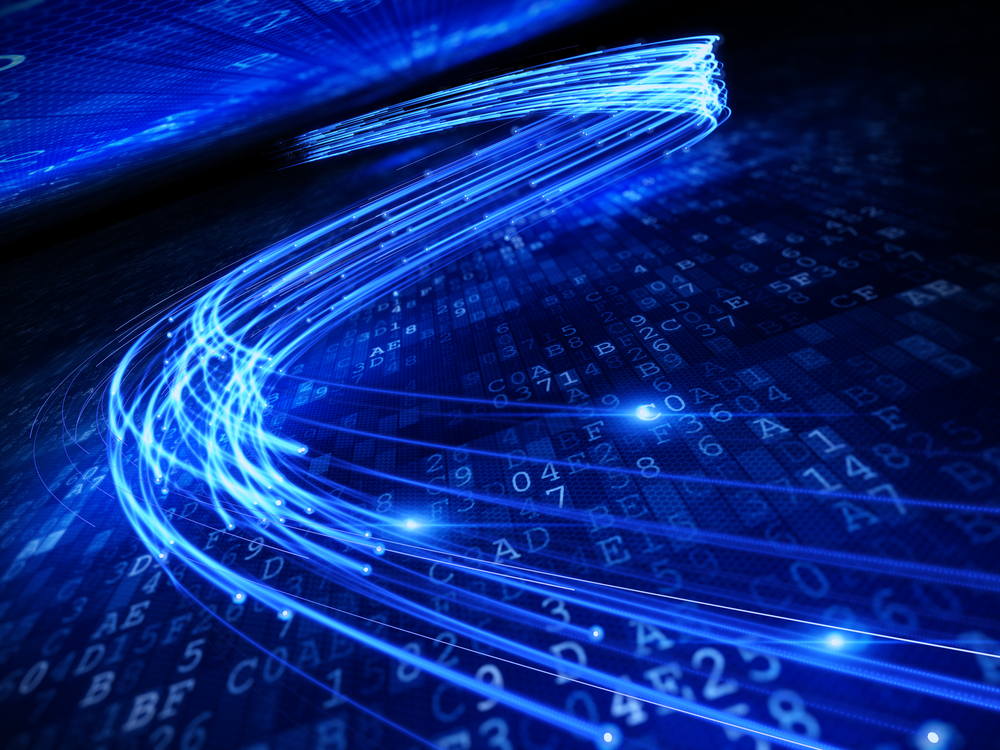
\includegraphics[width=\paperwidth, height=\paperheight]{wifi3}}

\addtobeamertemplate{block end}{}{\vspace*{2ex}} % White space under blocks
\addtobeamertemplate{block alerted end}{}{\vspace*{2ex}} % White space under highlighted (alert) blocks
\addtobeamertemplate{blockNT end}{}{\vspace*{2ex}} % White space under highlighted (alert) blocks
\setlength{\belowcaptionskip}{2ex} % White space under figures
\setlength{\belowdisplayshortskip}{2ex} % White space under equations

\begin{frame}[t] % The whole poster is enclosed in one beamer frame

\begin{columns}[t] % The whole poster consists of three major columns, the second of which is split into two columns twice - the [t] option aligns each column's content to the top

\begin{column}{\sepwid}\end{column} % Empty spacer column

\begin{column}{0.9\onecolwid} % The first column

%---------------------------------------------------------------
% Introduce the team
%---------------------------------------------------------------

%%%%%%%%%%%%%%%%%%%%%%%%%EDITEDIT
    \begin{mdframed}[backgroundcolor=white, userdefinedwidth=0.999999\linewidth]
    \centering
    \center
    \usebeamercolor{title in headline}{\color{ForestGreen}\Large{\textbf{\vspace{0.5cm} \\ Who are we? CHANGE THIS TO THE TITLE OF YOUR FIRST COLLUMN. \vspace{0.5cm}}}\\[0.5ex]}
    \end{mdframed}
    \vspace{1.75cm} % This increases the spacing between the blocks

%%%%%%%%%%%%%%%%%%%%%EDITEDIT
\begin{alertblock}{PhD Student BLOCK TITLE}
\begin{columns}
%\begin{column}{0.01\linewidth}
%\end{column} Uncomment this to create a spacing column
\begin{column}{0.65\linewidth}
BLOCK TEXT
\textbf{H. Wragg}

SAMBa aligned PhD student at the University of Bath.
\end{column}
\begin{column}{0.29\linewidth}
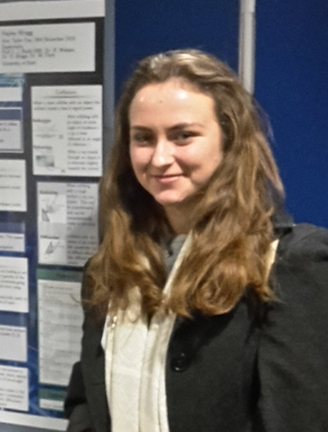
\includegraphics[scale=0.72]{HWragg.jpg} 
\end{column}
\end{columns}
\end{alertblock}
\vspace{1cm}

%%%%%%%%%%%%%%%%EDITEDIT
\begin{block}{Supervisors BLOCK TITLE}
\vspace{-2cm}
\begin{columns}
\begin{column}{0.25\linewidth}
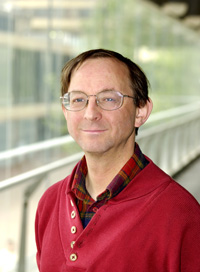
\includegraphics[scale=2.9]{chris-budd.jpg}
\end{column}
\begin{column}{0.75\linewidth}
BLOCK TEXT
\textbf{Primary Supervisor: \\ C. Budd}
 \\
Professor of Applied Mathematics at the University of Bath and Professor of Mathematics at the Royal Institution of Great Britain. \\
\end{column}
\end{columns}
\vspace{2cm}
\begin{columns}
\begin{column}{0.77\linewidth}
\textbf{Secondary Supervisor: \\ R. Watson}
 \\
Senior Lecturer in the department of Electronic and Electrical Engineering at the University of Bath. \\
\end{column}
\begin{column}{0.25\linewidth}
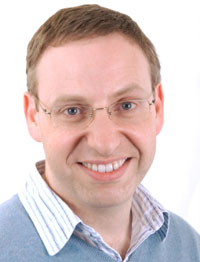
\includegraphics[scale=0.75]{RWatson.jpg}
\end{column}
\end{columns}
\end{block}
\vspace{1.75cm}

%%%%%%%%%%EDITEDIT
\begin{alertblock}{Industrial Supervisors BLOCK TITLE}
\begin{columns}
\begin{column}{0.24\linewidth}
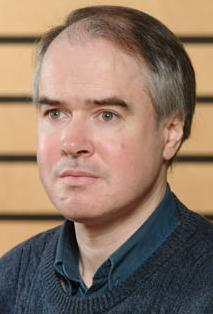
\includegraphics[scale=0.7]{KBriggs.jpg}
\end{column}
\begin{column}{0.74\linewidth}
BLOCK TEXT
\textbf{K. Briggs}
 \\
A research mathematician, for BT TSO at Adastral Park. \\
\end{column}
\end{columns}
\begin{columns}
\begin{column}{0.6\linewidth}
\textbf{M. Fitch}
 \\
A research engineer for BT TSO at Adastral Park. \\
\end{column}
\begin{column}{0.24\linewidth}
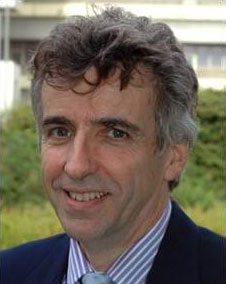
\includegraphics[scale=0.75]{MFitch.jpg}
\end{column}
\end{columns}
\end{alertblock}
 \hspace{0.5in}
 \begin{beamercolorbox}[wd=9in,colsep=0.15cm]{cboxb}
 \end{beamercolorbox}
 \vspace{0.1in}



%------------------------------------------------------------------------------
%		Introduce the location
%--------------------------------------------------------------------------------
    \begin{mdframed}[backgroundcolor=white, userdefinedwidth=0.999999\linewidth]
    \centering
    \center
    \usebeamercolor{title in headline}{\color{ForestGreen}\Large{\vspace{0.5cm}
    %%%%%%%%%%%%%%EDITEDIT
     \textbf{Where? TITLE} \vspace{0.5cm} }\\[0.5ex]}
    \end{mdframed}
    \vspace{1.5cm}
\begin{block}{
%%%%%%%%%%%EDITEDIT
Adastral Park BLOCK TITLE}
\begin{columns}
\begin{column}{0.6\linewidth}
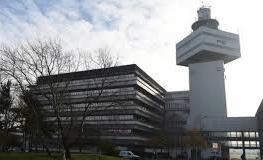
\includegraphics[scale=2]{AdastralPark.jpeg} \\ \end{column}
\begin{column}{0.3\linewidth}
BLOCK TEXT
Adastral Park is home to the research labs for BT.
\end{column}
\end{columns}
 \vspace{1cm}
%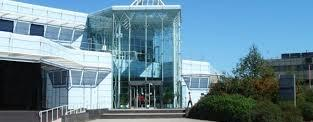
\includegraphics[scale=2.75]{AdastralPark2.jpg}
\end{block}

%---------------------------------------------------------------

\end{column} % End of the first column

\begin{column}{1.5\sepwid}\end{column} % Empty spacer column

\begin{column}{0.99\twocolwid} % Begin a column which is two columns wide (column 2)

%----------------------------------------------------------------------------------------
%	Introduce The Project
%----------------------------------------------------------------------------------------%
\begin{mdframed}[backgroundcolor=white, userdefinedwidth=0.999999\linewidth]
    \centering
    \center
    \usebeamercolor{title in headline}{\color{ForestGreen}\Large{\textbf{\vspace{0.5cm} \\ %%%%%%%%%%%%EDITEDIT
    The Project \vspace{0.5cm}}}\\[0.5ex]}
  
    \end{mdframed}
    \vspace{1.5cm}
    
\begin{alertblock}{\textbf{AIM} BLOCK TITLE
%%%%%%%%%%%%%%%%%%%EDITEDIT
}
BLOCK TEXT
\begin{itemize}
\item \textbf{Create an accurate model and reduce the time it takes to simulate indoor-to-indoor WiFi propagation in a domestic environment.}
\item \textbf{Use the model to optimize the location of low powered base stations.
}
\end{itemize}
\end{alertblock}
\vspace{-1cm}




%----------------------------------------------------------------------------------------
\begin{block}{Proposed method BLOCK TITLE
%%%%%%%%%%%%%%EDITEDIT
}
\vspace{-2cm}
BLOCK TEXT
\begin{itemize}
\item Use intelligent algorithms and adaptive mesh techniques to decrease execution time.
\item Compare simulation results to PDE models and to measured results from BT.
\item Develop a stochastic model for the environment.
\item Optimize the location of the transmitter using the developed model.
\end{itemize}
\end{block}
%----------------------------------------------------------------
%		MOTIVATION FOR THE RESEARCH
%------------------------------------------------------------
 
 \vspace{-2cm}
 \hspace{0.5in}
 \begin{beamercolorbox}[wd=14in,colsep=0.15cm]{cboxb}
 \end{beamercolorbox}
 \vspace{2cm}

\begin{alertblock}{High frequency BLOCK TITLE
%%%%%%%%%%%%%EDITEDIT
}
BLOCK TEXT
\begin{columns}
\begin{column}{0.05\linewidth}
\end{column}
\begin{column}{0.45\linewidth}
BLOCK TEXT
\begin{figure}[H]
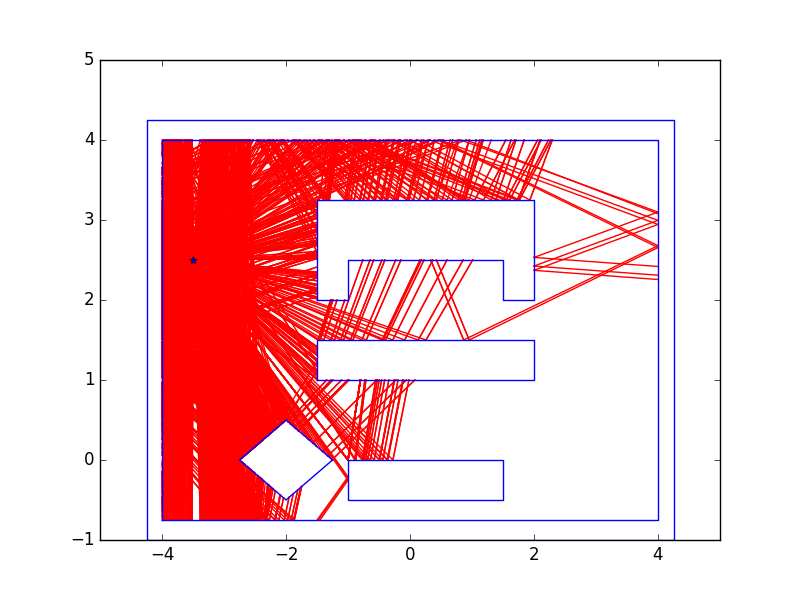
\includegraphics[scale=0.8]{MultiRay.jpg} 
\caption{The rays propagating from the transmitter.
%%%%%%%%%%%%%%%EDITEDIT
}
\end{figure}
\end{column}
\begin{column}{0.05\linewidth}
\end{column}
\begin{column}{0.45\linewidth}
%%%%%%%%%%%%%%EDITEDIT
BLOCK TEXT
\begin{itemize}
\item
Since the waves we are looking at are at a high frequency (typically of the order of 3GHz, but sometimes going higher)  we can model them using ray-tracing.
\item This is very computationally costly to run and requires lots of input information.
\end{itemize}
\end{column}
\end{columns}

\begin{columns}
\begin{column}{0.5\linewidth}
\begin{itemize}
%%%%%%%%%%%%%%%EDITEDIT
\item The signal strength can be calculated along the trajectory of the ray. 
\item This takes into account the loss from the distance travelled, and from the interactions with the furniture.
\end{itemize}
\end{column}
\begin{column}{0.45\linewidth}
\begin{figure}[H]
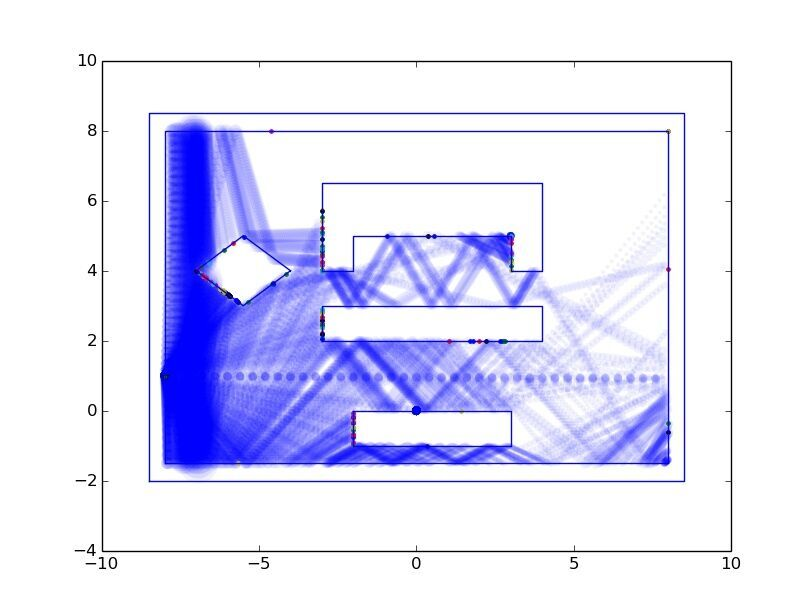
\includegraphics[scale=0.5]{signalcoverage2.jpeg} 
\caption{The signal strength along the ray trajectories.
%%%%%%%%%%%%%%%EDITEDIT
}
\end{figure}
\end{column}
\end{columns}
\end{alertblock}

%---------------------------------------------------------------------------
%		THE FOLLOWING SECTION SPLITS INTO ANOTHER TWO COLUMNS 
%----------------------------------------------------------------
%	Two columns to spilt Image and explanation
\begin{columns}
\begin{column}{0.45\linewidth}
\begin{block}{Domestic environment BLOCK TITLE}
\vspace{-1cm}
BLOCK TEXT
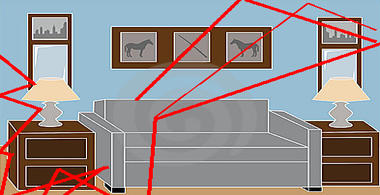
\includegraphics[scale=5.2]{livingroom.jpg} 
\end{block}
\end{column}

\begin{column}{0.01\linewidth}
% SPACER COLUMN
\end{column}

\begin{column}{0.45\linewidth}
\vspace{-1.25cm}
\begin{mdframed}[backgroundcolor=white, userdefinedwidth=0.999999\linewidth]
% THERE IS NO BLOCK TITLE HERE. TO CREATE ONE DELETE \begin{mdframed}[backgroundcolor=white, userdefinedwidth=0.999999\linewidth] AND \END{MDFRAMED} AND REPLACE WITH \BEGIN{BLOCK}{TITLE} AND \END{BLOCK}
\vspace{0.5cm}
BLOCK TEXT
\begin{itemize}
%%%%%%%%%%%%EDITEDIT
\item A domestic environment is very cluttered, which reduces the number of line-of-sight paths.
\item Each collision results in the wave having a combination of reflections, diffractions, and refractions. 
\end{itemize}
\vspace{0.5cm}
\end{mdframed}

\end{column}
\end{columns}

\end{column} % End of the second column

\begin{column}{\sepwid}\end{column} % Empty spacer column
\begin{column}{\sepwid}\end{column} % Empty spacer column
\begin{column}{1.1\threecolwid} % The third column


%----------------------------------------------------------------------------------------
%	RESEARCH METHODS
%-------%---------------------------------------------------------------


\begin{block}{Collisions BLOCK TITLE
%%%%%%%%%%%EDITEDIT
}
\vspace{-1.5cm}
%%%%%%%%%%%%%%EDITEDIT
BLOCK TEXT
Colliding with an object causes a loss in the signal power. 
\vspace{1.5cm}
\begin{columns}
\begin{column}{0.5\linewidth}
\textbf{Reflection} \\
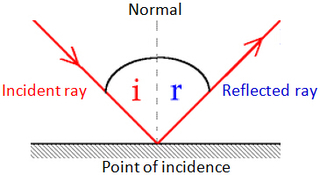
\includegraphics[scale=1]{Reflection.jpg} \cite{Reflection}
\end{column}
\begin{column}{0.5\linewidth}
%%%%%%%%%%%%%%%%EDITEDIT
 \\
 BLOCK TEXT
After colliding with an object at some angle of incidence $i$, a ray is then reflected at an angle of reflection $r$.
\end{column}
\end{columns}
\begin{columns}
\begin{column}{0.5\linewidth}
\textbf{Refraction} \\
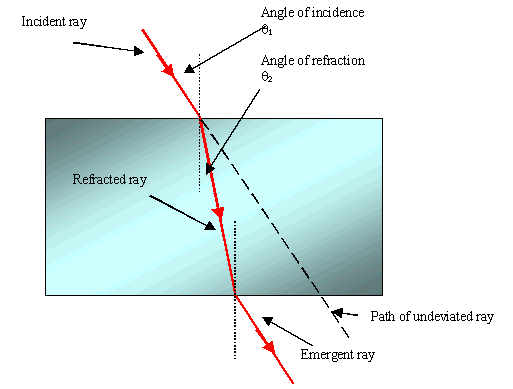
\includegraphics[scale=0.5]{Refraction.png} 
\cite{Refraction} 
\end{column}
\begin{column}{0.5\linewidth}
%%%%%%%%%EDITEDIT
BLOCK TEXT
When a ray travels through an object, it is refracted slightly towards the normal.
\end{column}
\end{columns}
\end{block}
\vspace{1.5cm}

% THIS BOX IS THE SAME COLOURS AS THE ALERTBOX BUT WITHOUT A TITLE
\begin{mdframed}[backgroundcolor=jblue!15, linecolor=jblue!70,
  linewidth=20pt,
  topline=true,
  rightline=true,
  leftline=true, bottomline=true, userdefinedwidth=0.999999999999999\linewidth]
  \begin{columns}
  \begin{column}{0.01\linewidth}
  \end{column}
  \begin{column}{0.445\linewidth}
 \vspace{0.5cm}
\textbf{Scattering
%%%%%%%%%%EDITEDIT
} \\
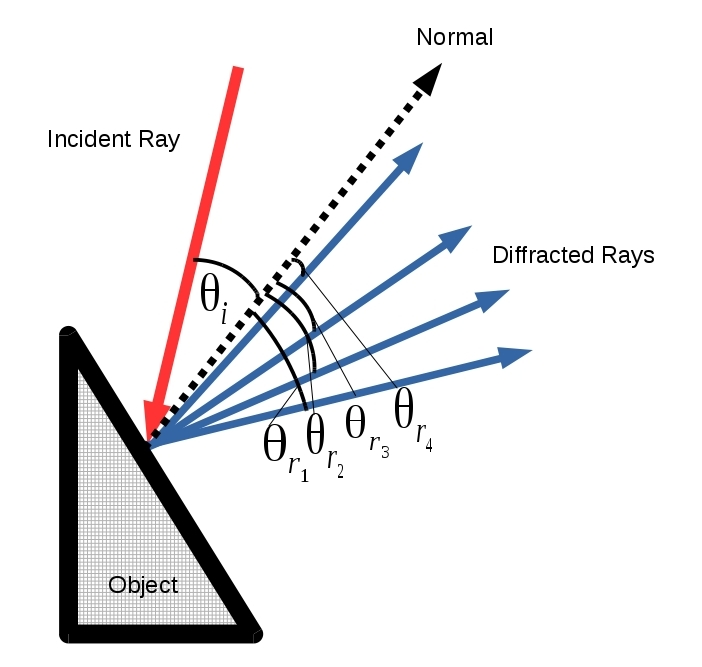
\includegraphics[scale=0.47]{Scattering.jpg} 
\\   
\end{column}

\begin{column}{0.52\linewidth}
 \vspace{0.5cm}
 \par
 %%%%%%%%%%%%%%%EDITEDIT
 BLOCK TEXT
When colliding with a rough surface, a ray can scatter. This can be unpredictable, and can be computationally costly to simulate. \cite{Antennas2007}
 \end{column}
 \end{columns}
 \vspace{1cm}
 \begin{columns}
 \begin{column}{0.01\linewidth}
  \end{column}
\begin{column}{0.445\linewidth}
\textbf{Diffraction
%%%%%%%%%%%EDITEDIT
} \\
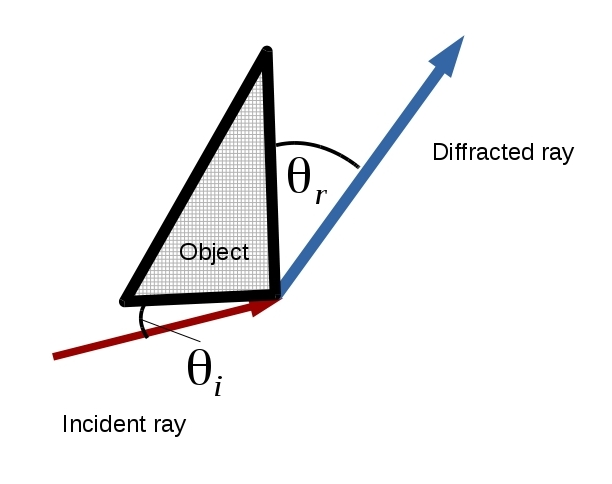
\includegraphics[scale=0.53]{Diffraction.jpg}
\end{column}
\begin{column}{0.53\linewidth}
BLOCK TEXT 
%%%%%%%%%%%EDITEDIT
Collision with the corner of an object causes the ray to diffract, which is also difficult to predict.
\end{column}
\end{columns}
\end{mdframed}


%----------------------------------------------------------------------------------------
%----------------------------------------------------------------------------------------

-------------------------------------
%	OBSERVATIONS
%----------------------------------------------------------------------------------------
% \begin{alertblock}{Observations}
%\end{alertblock}
%----------------------------------------------------------------------------------------
%----------------------------------------------------------------------------------------

-------------------------------------
%	RESULTS
%----------------------------------------------------------------------------------------
% \begin{block}{Results}
%\end{block}
%----------------------------------------------------------------------------------------
%----------------------------------------------------------------------------------------

-------------------------------------
%	CONCLUSIONS
%----------------------------------------------------------------------------------------


% \begin{alertblock}{Conclusions}
% What is the outcome of the work and what can be done in the future.
% \end{block}

%----------------------------------------------------------------------------------------
%----------------------------------------------------------------------------------------
%	REFERENCES
%----------------------------------------------------------------------------------------
\setbeamercolor{block alerted title}{fg=black,bg=CadetBlue} % Change the alert block title colors
\setbeamercolor{block alerted body}{fg=black,bg=white} % Change the alert block body colors
\vspace{1.5cm}
\begin{alertblock}{References}

\nocite{*} % Insert publications even if they are not cited in the poster
\tiny{\scalebox {.2}{\bibliographystyle{unsrt}}
%%%%%%EDITEDIT
 \bibliography{posterattempt1.bib}
 % Change the posterattempt1.bib file to change the references. The corresponding \cite{} calls will also need to be changed.
 \vspace{0.4in}}

\end{alertblock}


%----------------------------------------------------------------------------------------
%	ACKNOWLEDGEMENTS
%----------------------------------------------------------------------------------------

% \begin{block}{Acknowledgements}

% \end{block}

%---------------------------------------------------------------

\end{column} % End of the third column

\end{columns} % End of all the columns in the poster

\end{frame} % End of the enclosing frame

\end{document}
